\section{Results}
\label{section:results}

In order to demonstrate the performance of our method, we conducted two sets
of tests.
In the first we simulated observables from a set of stellar parameters for a
few hundred stars using the MIST stellar evolution models and the
gyrochronology model of equation \ref{eqn:gyro}.
The ages predicted with our model were compared to the true parameters used to
generate the data.
In the second we tested our model by measuring the ages of individual stars in
the NGC 6819 open cluster.

\subsection{Test 1: simulated stars}
For the first test we drew masses, ages, bulk metallicities, distances and
extinctions at random for 1000 stars from the following uniform distributions:
\begin{eqnarray}
& \mathrm{EEP} \sim U(198, 480) \\
% & M \sim U(0.5, 1.5)~[M_\odot] \\
& A \sim U(0.5, 14)\mathrm{~[Gyr]} \\
& F \sim U(-0.2, 0.2) \\
& D \sim U(10, 1000)~\mathrm{[pc]} \\
& A_V \sim U(0, 0.1).
\end{eqnarray}
\teff, \logg, \fhat, parallax, and apparent magnitudes $B$, $V$, $J$, $H$, $K$,
\gaia\ $G$, $G_{BP}$ and $G_{RP}$ were generated from these
stellar parameters using the MIST stellar evolution models.
We added a small amount of noise to the `observed' stellar properties in order
to reflect typical observational uncertainties.
We added Gaussian noise with a standard deviation of 25 K to \teff, 0.01 dex
to \feh\ and \logg, and 10 mmags to $B$, $V$, $J$, $H$, and $K$ magnitudes.
The noise added to Gaia $G$-band photometry ranged from
0.3 mmag for stars brighter than 13th magnitude, to 10 mmag for stars
around 20th magnitude \citep{evans2017, brown2018}.
Noise added to \gaia\ $G_{BP}$ and $G_{RP}$ bands ranged from 2 mmag for stars
brighter than 13th magnitude to 200 mmag for stars fainter than 17th.
Unphysical combinations of stellar parameters were discarded, resulting in a
final sample size of 841 simulated stars.
Figure \ref{fig:CMD_age} shows the position of these stars on an HRD
(with \logg\ on the y-axis instead of luminosity to improve the visibility of
the MS), colored by their age.
Rotation periods for these stars were generated using the gyrochronology
relation described in equation \ref{eqn:gyro}.
We added 5\% Gaussian noise to all stellar rotation periods to represent
measurement uncertainties of 5\%.
The median uncertainty on rotation periods calculated from \kepler\ light
curves using an autocorrelation function mnethod, provided in the
\citet{mcquillan2014} catalog is 1\%.
However, the \citet{aigrain2015} injection and recovery study showed that true
rotation period uncertainties are often slightly larger than this.
A Gaussian is a crude approximation for the noise distribution of rotation
periods which can be highly non-Gaussian \citep[\eg][]{aigrain2015,
angus2018}.
\begin{figure}
  \caption{
      The simulated star sample plotted on an HRD, colored by age
    (top panel) and rotation period (bottom panel).
    HRD positions were calculated using MIST isochrones via the {\tt
    isochrones.py} {\it Python} package and rotation periods were generated
    using equation \ref{eqn:gyro}.
    This figure was generated in a Jupyter notebook available at
    \url{https://github.com/RuthAngus/stardate/blob/master/paper/code/Simulate_data.ipynb}
}
  \centering
    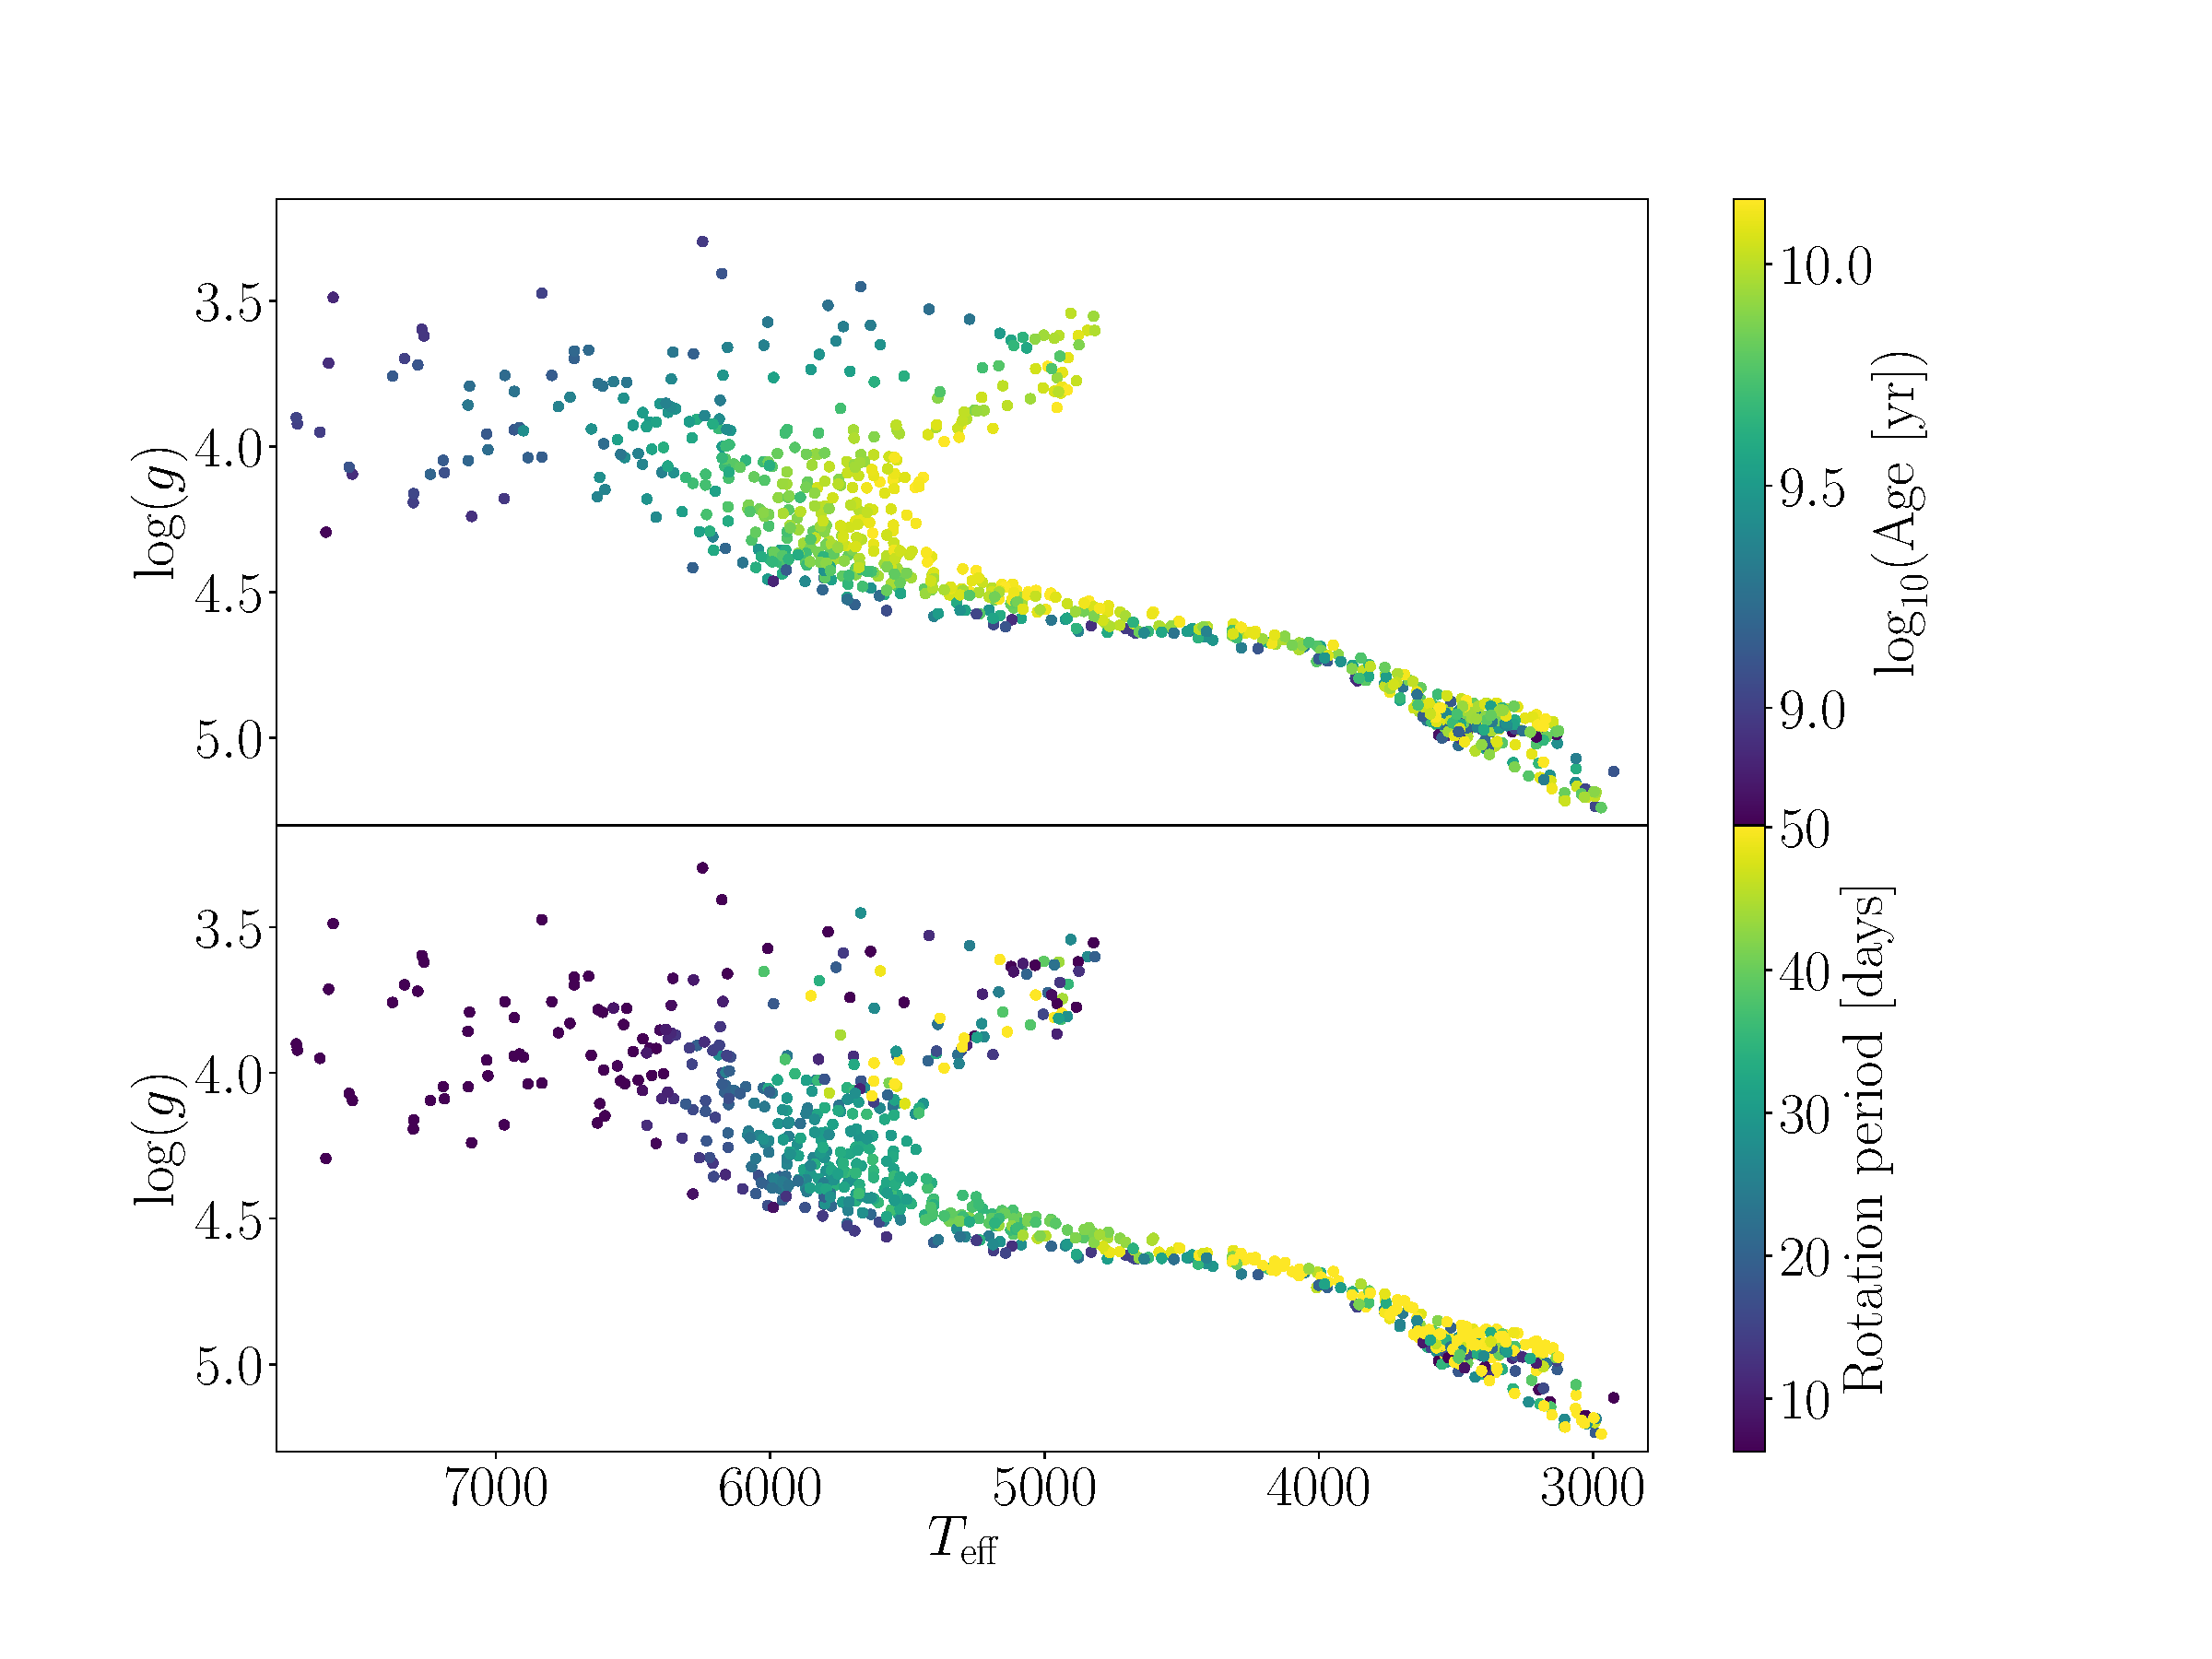
\includegraphics[width=1\textwidth]{simulated_CMD}
\label{fig:CMD_age}
\end{figure}
Figure \ref{fig:rotation_model} shows the rotation periods of 841
stars generated from the gyrochronology model.
\begin{figure}
  \caption{
The rotation period model.
    Late F, GK and early M dwarfs (stars with 0.56 $<$ \gcolor\ $<$ 2.7 follow
    the Praesepe-calibrated gyrochronology relation (dashed gray lines), with
    the exception of old, slowly
    rotating stars with large Rossby numbers whose rotation periods are fixed
    at 2$\times$ their convective overturn time.
    The rotation periods of early F (\gcolor $<$ 0.56), late M dwarfs (\gcolor
    $<$ 2.7) and subgiants (EEP $>$ 454) were generated
    from a log-normal distribution with standard deviation shown in figure
    \ref{fig:variance}.
% The top panel shows the rotation periods vs. B-V colors of simulated stars,
The top panel shows the rotation periods vs. \gcolor\ colors of simulated stars,
    colored by their age and the bottom panel shows the same stars colored
    by their equivalent evolutionary point (EEP).
    % 9, 11, and 13 (rotation periods rise with age).
    The gray lines describe the mean gyrochronology model at ages 1,
    3, 5, 7, 9, 11, and 13 (rotation periods rise with age).
}
  \centering
    \includegraphics[width=1.\textwidth]{rotation_model_praesepe}
\label{fig:rotation_model}
\end{figure}

We took two approaches to inferring the ages of these simulated stars:
firstly using isochrone fitting {\it only}, and secondly using isochrone
fitting {\it combined with} a gyrochronology model (\sd).
Since the posterior PDFs of stars are often multimodal, we found that the
choice of initial positions of the {\tt emcee} walkers influenced the final
outcome because walkers occasionally got stuck in local minima.
We found that the following set of initial parameters worked well, though not
perfectly: EEP = 330, $A = 9.56$ Gyr, $F = -0.05$, $D = 269$ pc and $A_V =
0.0$.
Figure \ref{fig:simulation_results} shows the results of combining
gyrochronology with isochrone fitting for the simulated sample.
The stars' true ages are plotted against their predicted ages, with ages
inferred with gyrochronology and isochrone fitting
in color, and ages inferred using isochrone fitting only plotted in light
grey.
\racomment{
    The different panels show the results for different types of stars: FGK
dwarfs that are still undergoing magnetic braking, FGK dwarfs that have ceased
magnetic braking (their Rossby number is around 2), M dwarfs, and evolved
stars.
The selection criteria for these groups are in the panel headings.
The FGK dwarfs with low Rossby numbers showed the largest improvement: the
median age precision for this group (defined as the standard deviation of the
posterior as a percentage of the median age) was 11\% when using a combination
of isochrones and gyrochronology, and 32\% using isochrone fitting alone.
The age RMS of this group was 0.9 Gyr using isochrones and gyrochronology, and
3.4 Gyr using isochrones only.
This equates to a 3$\times$ improvement in age precision.
Despite the fact that stars with Rossby numbers of 2 have stopped spinning
down and their rotation periods no longer evolve with age, their rotation
periods are {\it still age informative}.
This is because their rotation periods are still directly related to their
age, but also {\it indirectly} related to their age via EEP and metallicity,
as shown in equation \ref{eqn:gyro}.
When including rotation periods to infer the ages of stars with large Rossby
numbers, age precision improves from 21\% to 11\% and the age RMS improves
from 2.5 to 0.9 Gyr.
% Age precision also increases for F dwarfs when incorporating their rotation
% periods, even though they are not directly related to their ages.
% This is because rotation period relates to color via the variance model in
% equation \ref{eqn:gyro}.
The precision of M dwarf ages did improve overall when their rotation periods
were included, but this improvement was entirely driven by the early M dwarfs.
The precision of this group improved from 56\% to 25\% and RMS from 4.5 Gyr
to 3.8 Gyr.
The precision of ages inferred for evolved stars changed very little when
rotation periods were included in the inference process.
This is because the variance of the rotation-age relation was inflated by a
large amount in the gyrochronology model (equation \ref{eqn:gyro}), making
rotation periods almost entirely uninformative for this group.
}
\begin{figure}
  \caption{
The true vs. predicted ages of simulated stars.
    Ages calculated by combining gyrochronology
    and isochrone fitting with \sd are shown in color and ages calculated with
    isochrone fitting only are shown in gray.
The different panels show the results for stars
    with \gcolor\ $<$ 2.2 (FGK dwarfs) that are still braking magnetically
    ($Ro < 2$), stars with \gcolor\ $<$ 2.2 that have stopped braking
    magnetically ($Ro \geq 2$),
    stars with 2.2 $<$ \gcolor\ (M dwarfs), and evolved stars (EEP $>$ 420).
Gyrochronology is highly effective for FGK stars: ages inferred with both
    gyrochronology and isochrone fitting are more accurate and precise than
    ages inferred via isochrone fitting only for this group.
Neither gyrochronology nor isochrone fitting can provide precise ages for
    M dwarfs, so the ages of these stars are imprecise regardless of
    age-dating method.
}
  \centering
    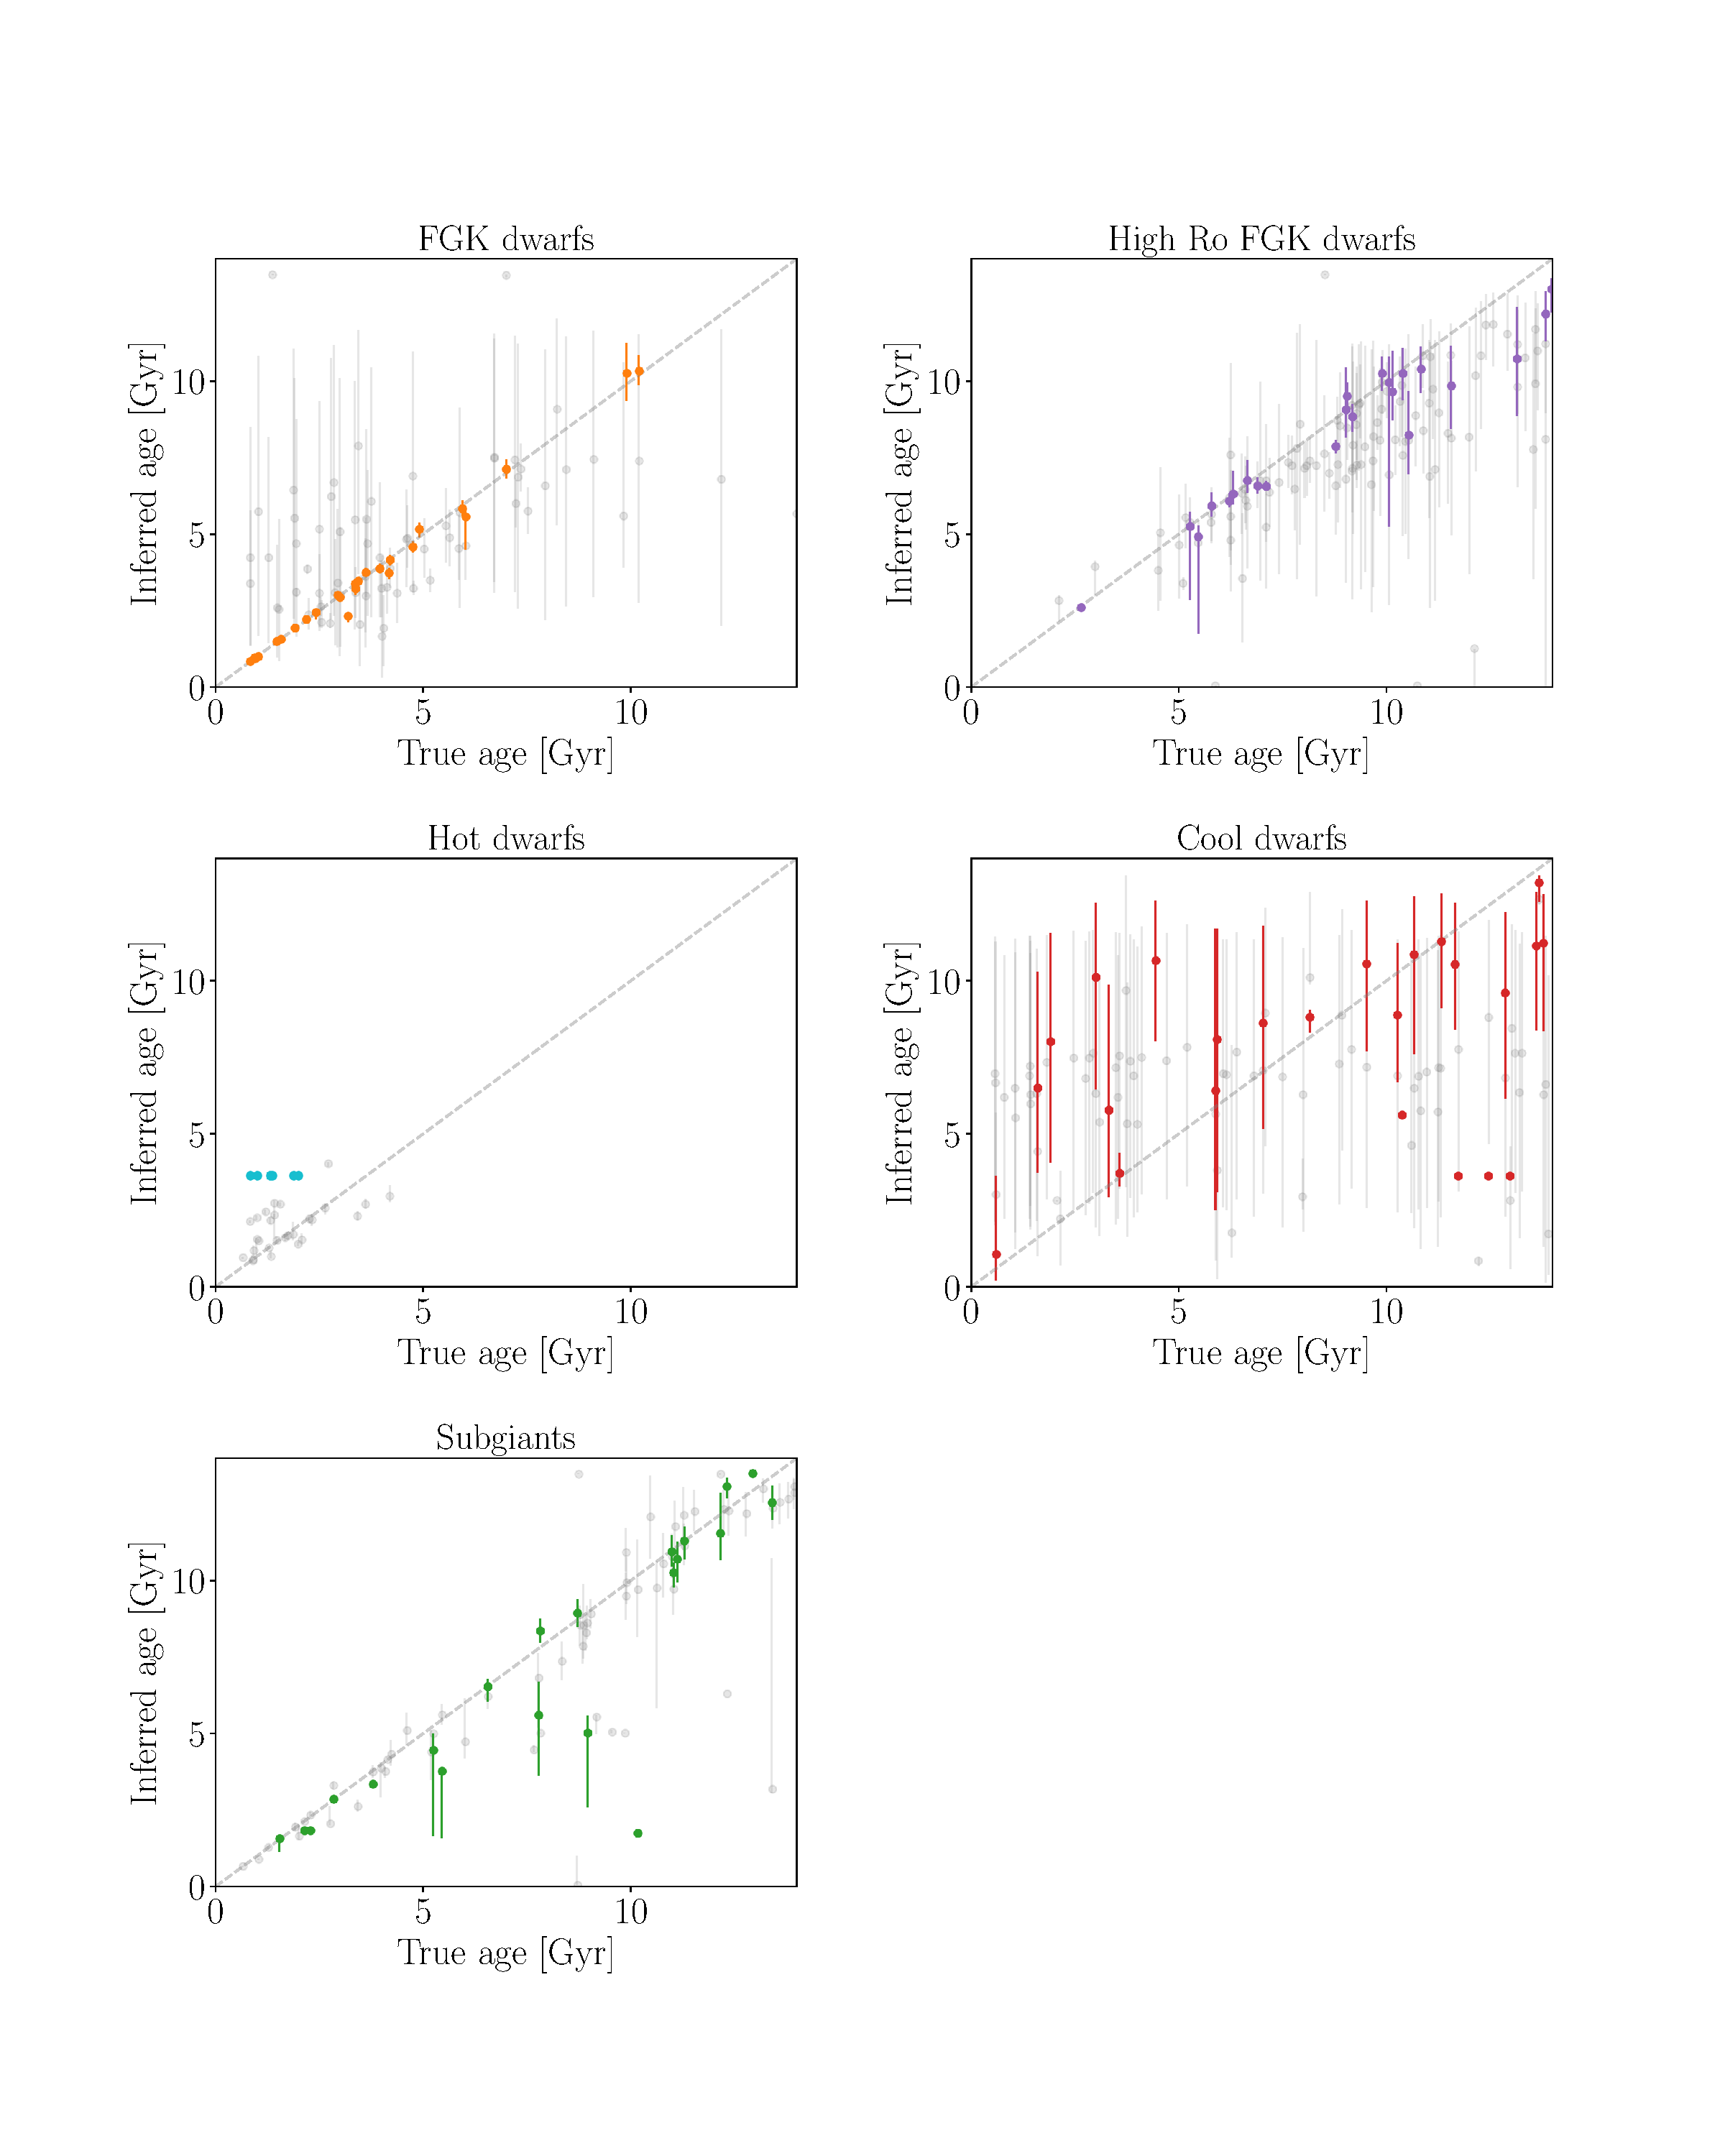
\includegraphics[width=1\textwidth]{simulation_results}
\label{fig:simulation_results}
\end{figure}

% Figure \ref{fig:all_iso_gyr} shows the inferred vs. true ages of all simulated
% stars, colored by their \gaia\ \gcolor\ age.
% The ages of FGK stars (\gcolor\ $<$ 2.2) were more precisely recovered with
% gyrochronology and isochrone fitting than with isochrone fitting alone.
% In both cases M dwarfs ages were not precisely recovered.
% \begin{figure}
%   \caption{
%       Inferred vs. true ages for all simulated stars using isochrones plus
%       gyrochronology via the \sd\ code (left) and isochrones only (right).
%       Stellar ages are colored by \gaia\ \gcolor\ color.
%       The ages of FGK stars (\gcolor\ $<$ 2.2)
%       were more precisely recovered with \sd\ than with isochrones only.
%       In both cases M dwarfs ages were not precisely recovered.
%       Points in the lower right of the left panel are either M dwarfs or
%       evolved (EEP $>$ 400).
%       In both panels, the ages of FGK stars were slightly underestimated.
% }
%   \centering
%     \includegraphics[width=1\textwidth]{all_iso_gyro}
% \label{fig:all_iso_gyro}
% \end{figure}

\racomment{
Figure \ref{fig:eep} shows the inferred equivalent evolutionary point (EEP)
for the simulated star sample.
EEP is a dimensionless number that describes evolutionary stage and, combined
with age and metallicity, determines stellar mass.
An interesting result of inferring stellar properties with both isochrones
{\it and} rotation periods is an increase in EEP precision.
The reason for this is partly that EEP and age are correlated, so shrinking
the age posterior also shrinks the EEP posterior, and partly because rotation
period is a function of HRD position.
As shown in equation \ref{eqn:gyro}, rotation period does not just depend on
color and age, but also on EEP and [Fe/H].}
\begin{figure}
  \caption{
    Inferred EEP for the simulated star sample with isochrones plus
    gyrochronology (left panel) and isochrone fitting only (right panel).
    Rotation periods provide information about position on the HRD via
equation \ref{eqn:gyro} and therefore improve all stellar parameters, not
just age.
}
  \centering
    \includegraphics[width=1\textwidth]{eep}
\label{fig:eep}
\end{figure}

Figure \ref{fig:precision} shows the simulated stars on an HRD, with
points colored by the precision of their predicted ages
(defined as the standard deviation of the age
posterior PDF, as a percentage of the median age).
The top panel shows the precision of ages calculated using both gyrochronology
and isochrone fitting via \sd\ and the bottom panel shows the precision of
ages calculated with isochrone fitting only.
Although these are empirical uncertainties, calculated via MCMC which only
approximates the age posterior PDFs, they show that combining gyrochronology
and isochrone fitting improves age precision on the MS.
\begin{figure}
  \caption{
Simulated stars on an HRD, colored by their relative age precision
    using gyrochronology and isochrone fitting via \sd\ (top panel) and
    isochrone fitting only (bottom panel).
Combining gyrochronology with isochrone fitting significantly improves stellar
    age precision on the MS.
Isochrone fitting provides precise ages for hot stars and subgiants and the
    rotation periods of these stars are relatively uninformative, so
    gyrochronology does not significantly improve their age precision.
The ages of late M dwarfs are highly imprecise because their ages are not well
    determined by either their rotation periods or their position on the HRD
    or CMD.
}
  \centering
    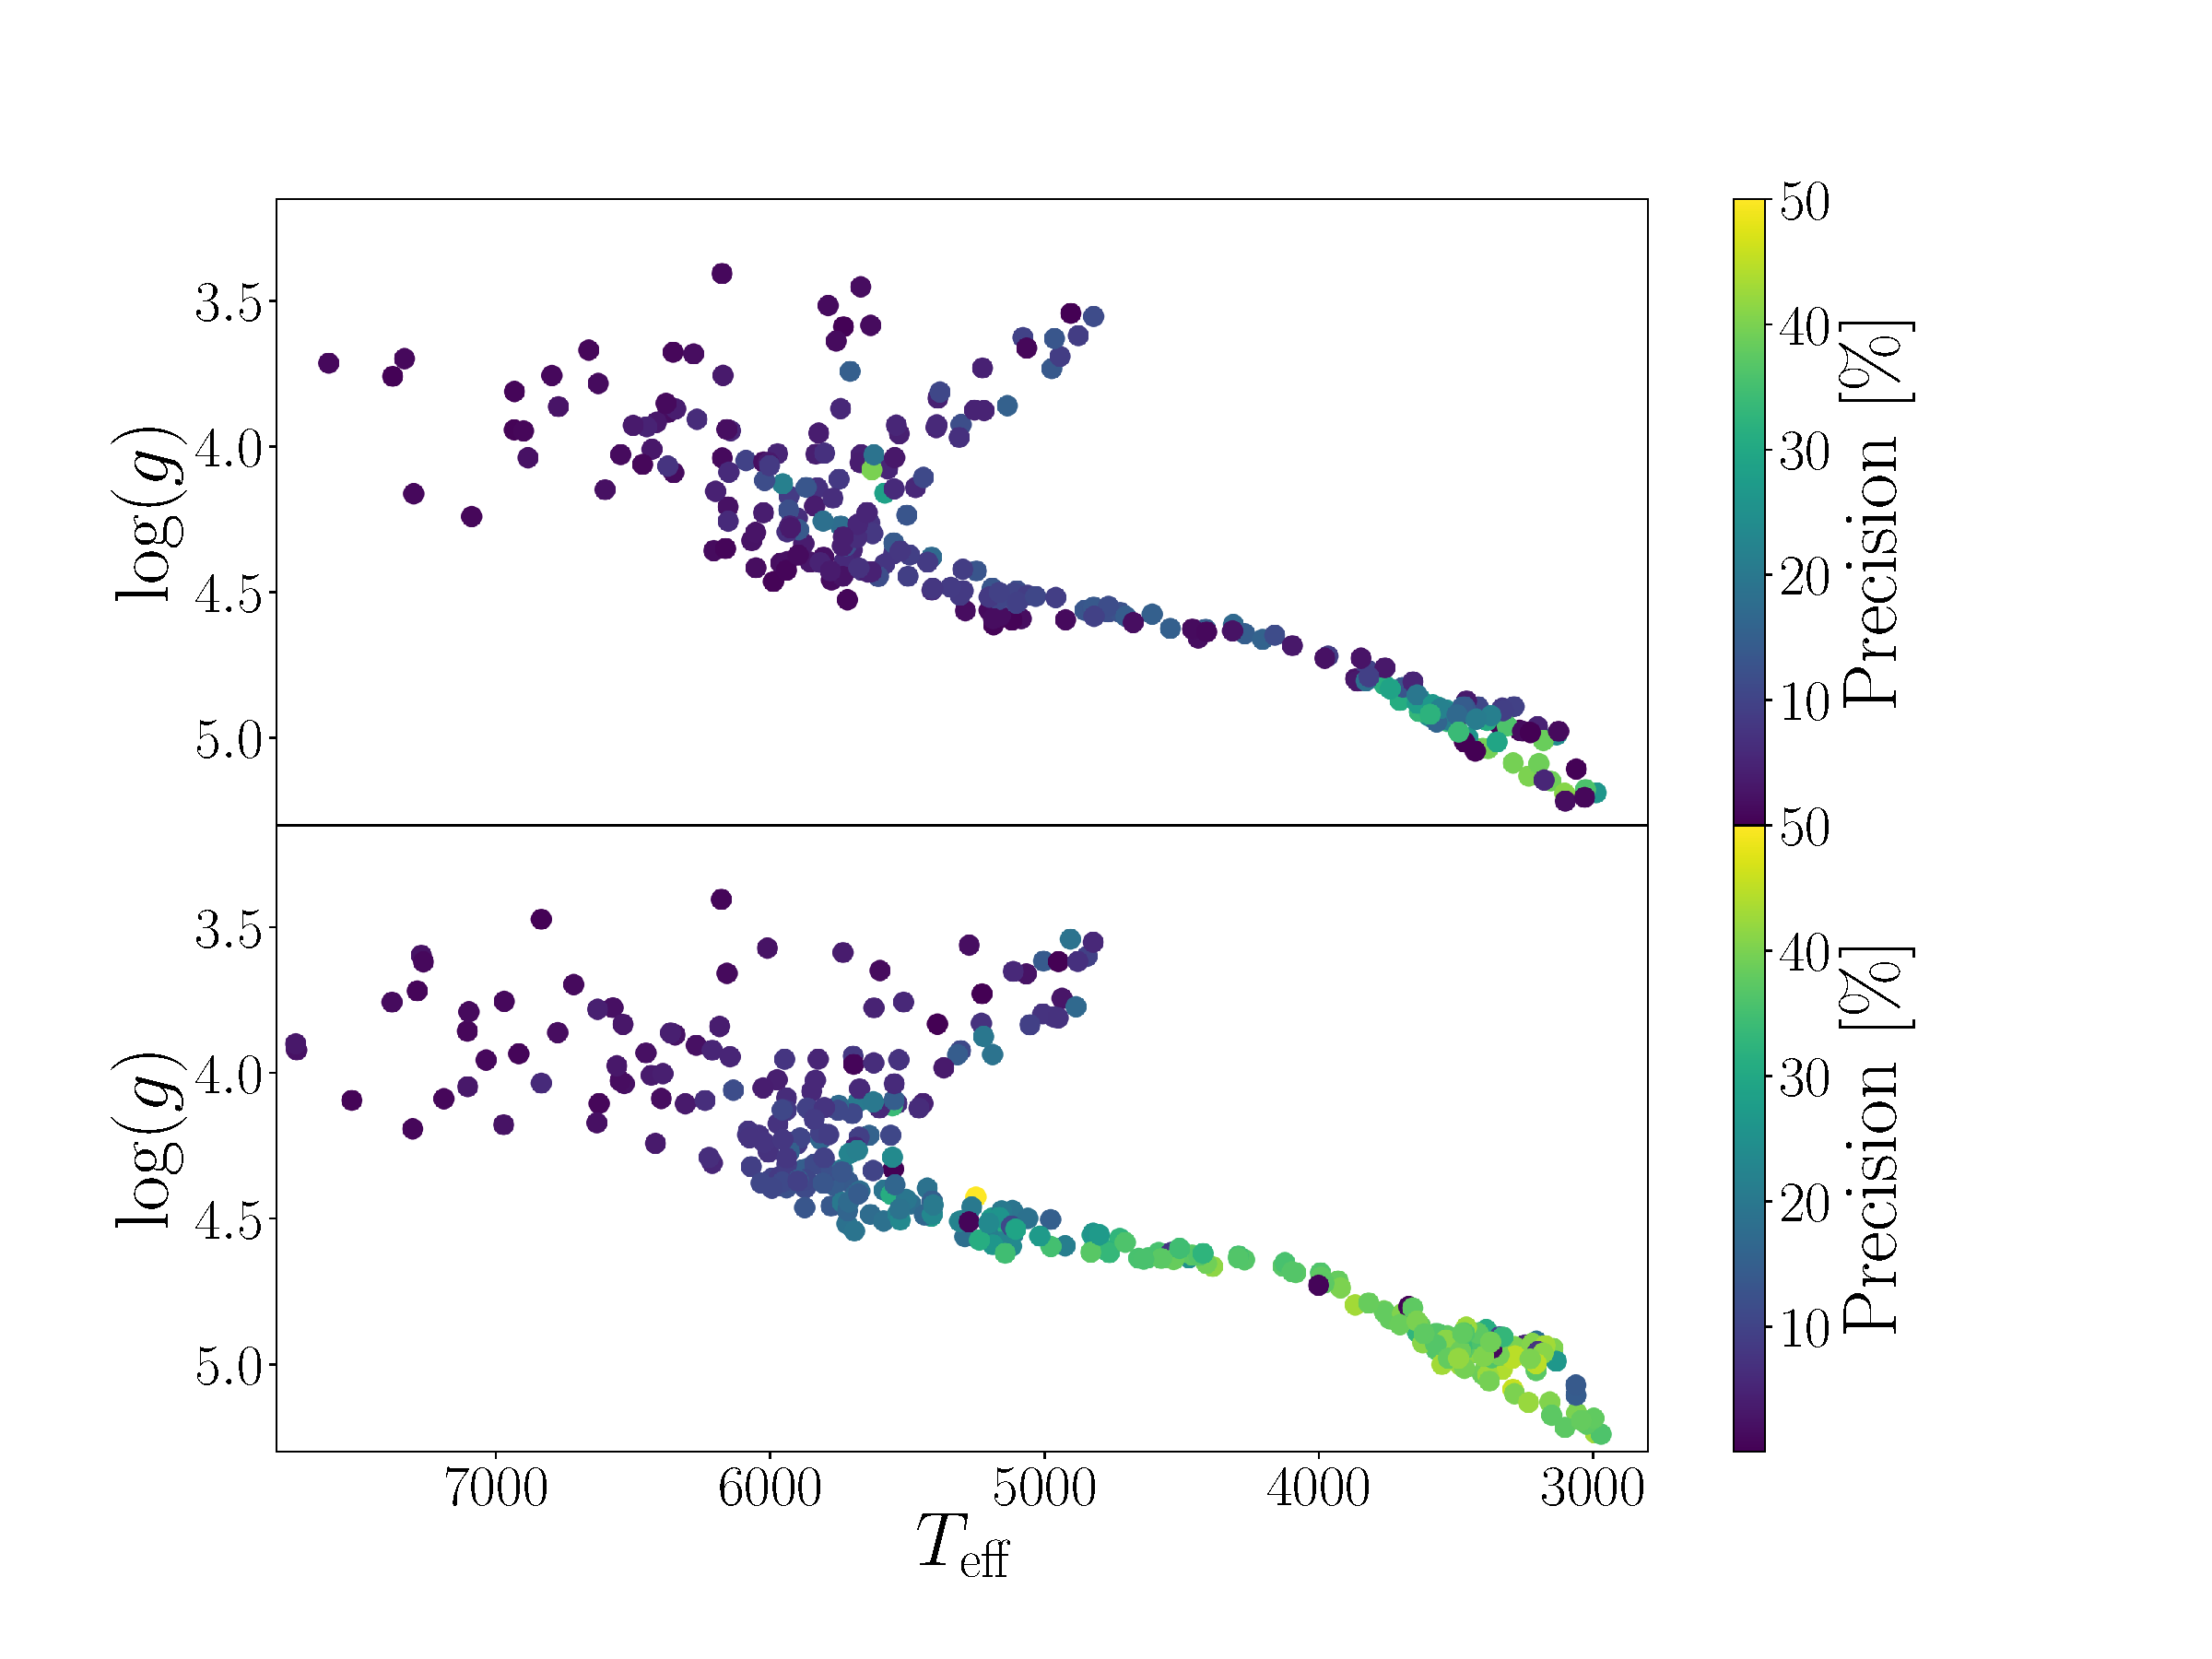
\includegraphics[width=1\textwidth]{precision_plot}
\label{fig:precision}
\end{figure}

\racomment{
This simulation experiment was designed to show the theoretical improvement in
age precision when gyrochronology is incorporated into isochrone fitting.
However, it does not demonstrate the accuracy of this method because the test
data were simulated from the same model used to infer ages.
The results of this experiment are therefore extremely accurate by design.
When applying this method to real data, the results will only be accurate if
the model is accurate.
In other words, \sd, like any age-dating method, provides model-dependent
ages.
Stellar ages calculated with \sd\ depend on both the accuracy of the MIST
models {\it and} the accuracy of the gyrochronology model (equation
\ref{eqn:gyro}).
In order to test the accuracy of \sd, we applied it to real data, as described
in the following section.}

\subsection{Test 2: Open clusters}
\racomment{
In order to test our model on real stars with known ages, we selected a sample
of stars in the 2.5 Gyr NGC 6819 cluster.
We compiled \kepler-based rotation periods \citep{meibom2015}, \Gaia\
photometry and \gaia\ parallaxes for members of the NGC 6819 cluster.
Figure \ref{fig:NGC6819} shows the period-color relation of this
cluster and figure \ref{fig:NGC6819_results} shows the results of inferring
the ages of individual cluster members using a combination of gyrochronology
and isochrone fitting (via \sd) and isochrone fitting alone.
The ages of F stars in this cluster (\gcolor\ $\sim$ 5.5-6.5) were relatively
precisely constrained by isochrone fitting alone because, at 2.5 Gyr, they are
approaching MS turn-off.
For these hot stars, ages inferred with gyrochronology and isochrones were
similar to ages inferred with isochrones and similarly precise, showing that
isochrones provide a lot of age information for these stars and rotation
periods do not add significantly more information.
The G and early K stars in this cluster (\gcolor\ $\lesssim$ .65) were not
precisely recovered from isochrone fitting alone -- the isochrone-only age
posteriors tend towards the prior which is a uniform distribution between 0
and 13.8 Gyrs.
The median age of stars in the cluster was 4.27 $\pm$ 0.48 Gyr when only
isochrone fitting was used.
In contrast, including gyrochronology when inferring the ages of G and K stars
in this cluster significantly improved age precision.
The median age of stars in this cluster was 2.63 $\pm$ 0.16 Gyr when ages were
inferred with a combination of isochrone fitting and gyrochronology, using the
newly calibrated Praesepe-based gyrochronology model.
The previously-calibrated \citet{angus2015} model resulted in a median stellar
age of 2.66 $\pm$ 0.21 Gyr, which is still consistent with the established
cluster age of 2.5 Gyr.
The median age of stars in the cluster using uncorrected photometry was
slightly underestimated at 1.86 $\pm$ 0.22 Gyr.
This suggests that, despite the fact that V-band extinction is marginalized
over during the inference process, correcting for extinction {\it before} ages
are estimated will reduce bias introduced by dust.
}
\begin{figure}
  \caption{
    The \kepler-based rotation periods of members of the 2.5 Gyr NGC 6819 open
    cluster.
    The raw \gcolor\ colors are shown in red and the dust-corrected colors are
    shown in black.
    The dashed line shows a gyrochronology model that was fit to the Praesepe
    cluster and the Sun in this work, interpolated to 2.5 Gyrs.
    This model was used to infer the ages of these stars.
    For comparison, the solid blue line shows a previously calibrated
    gyrochronology model \citep{angus2015}.
  }
  \centering
    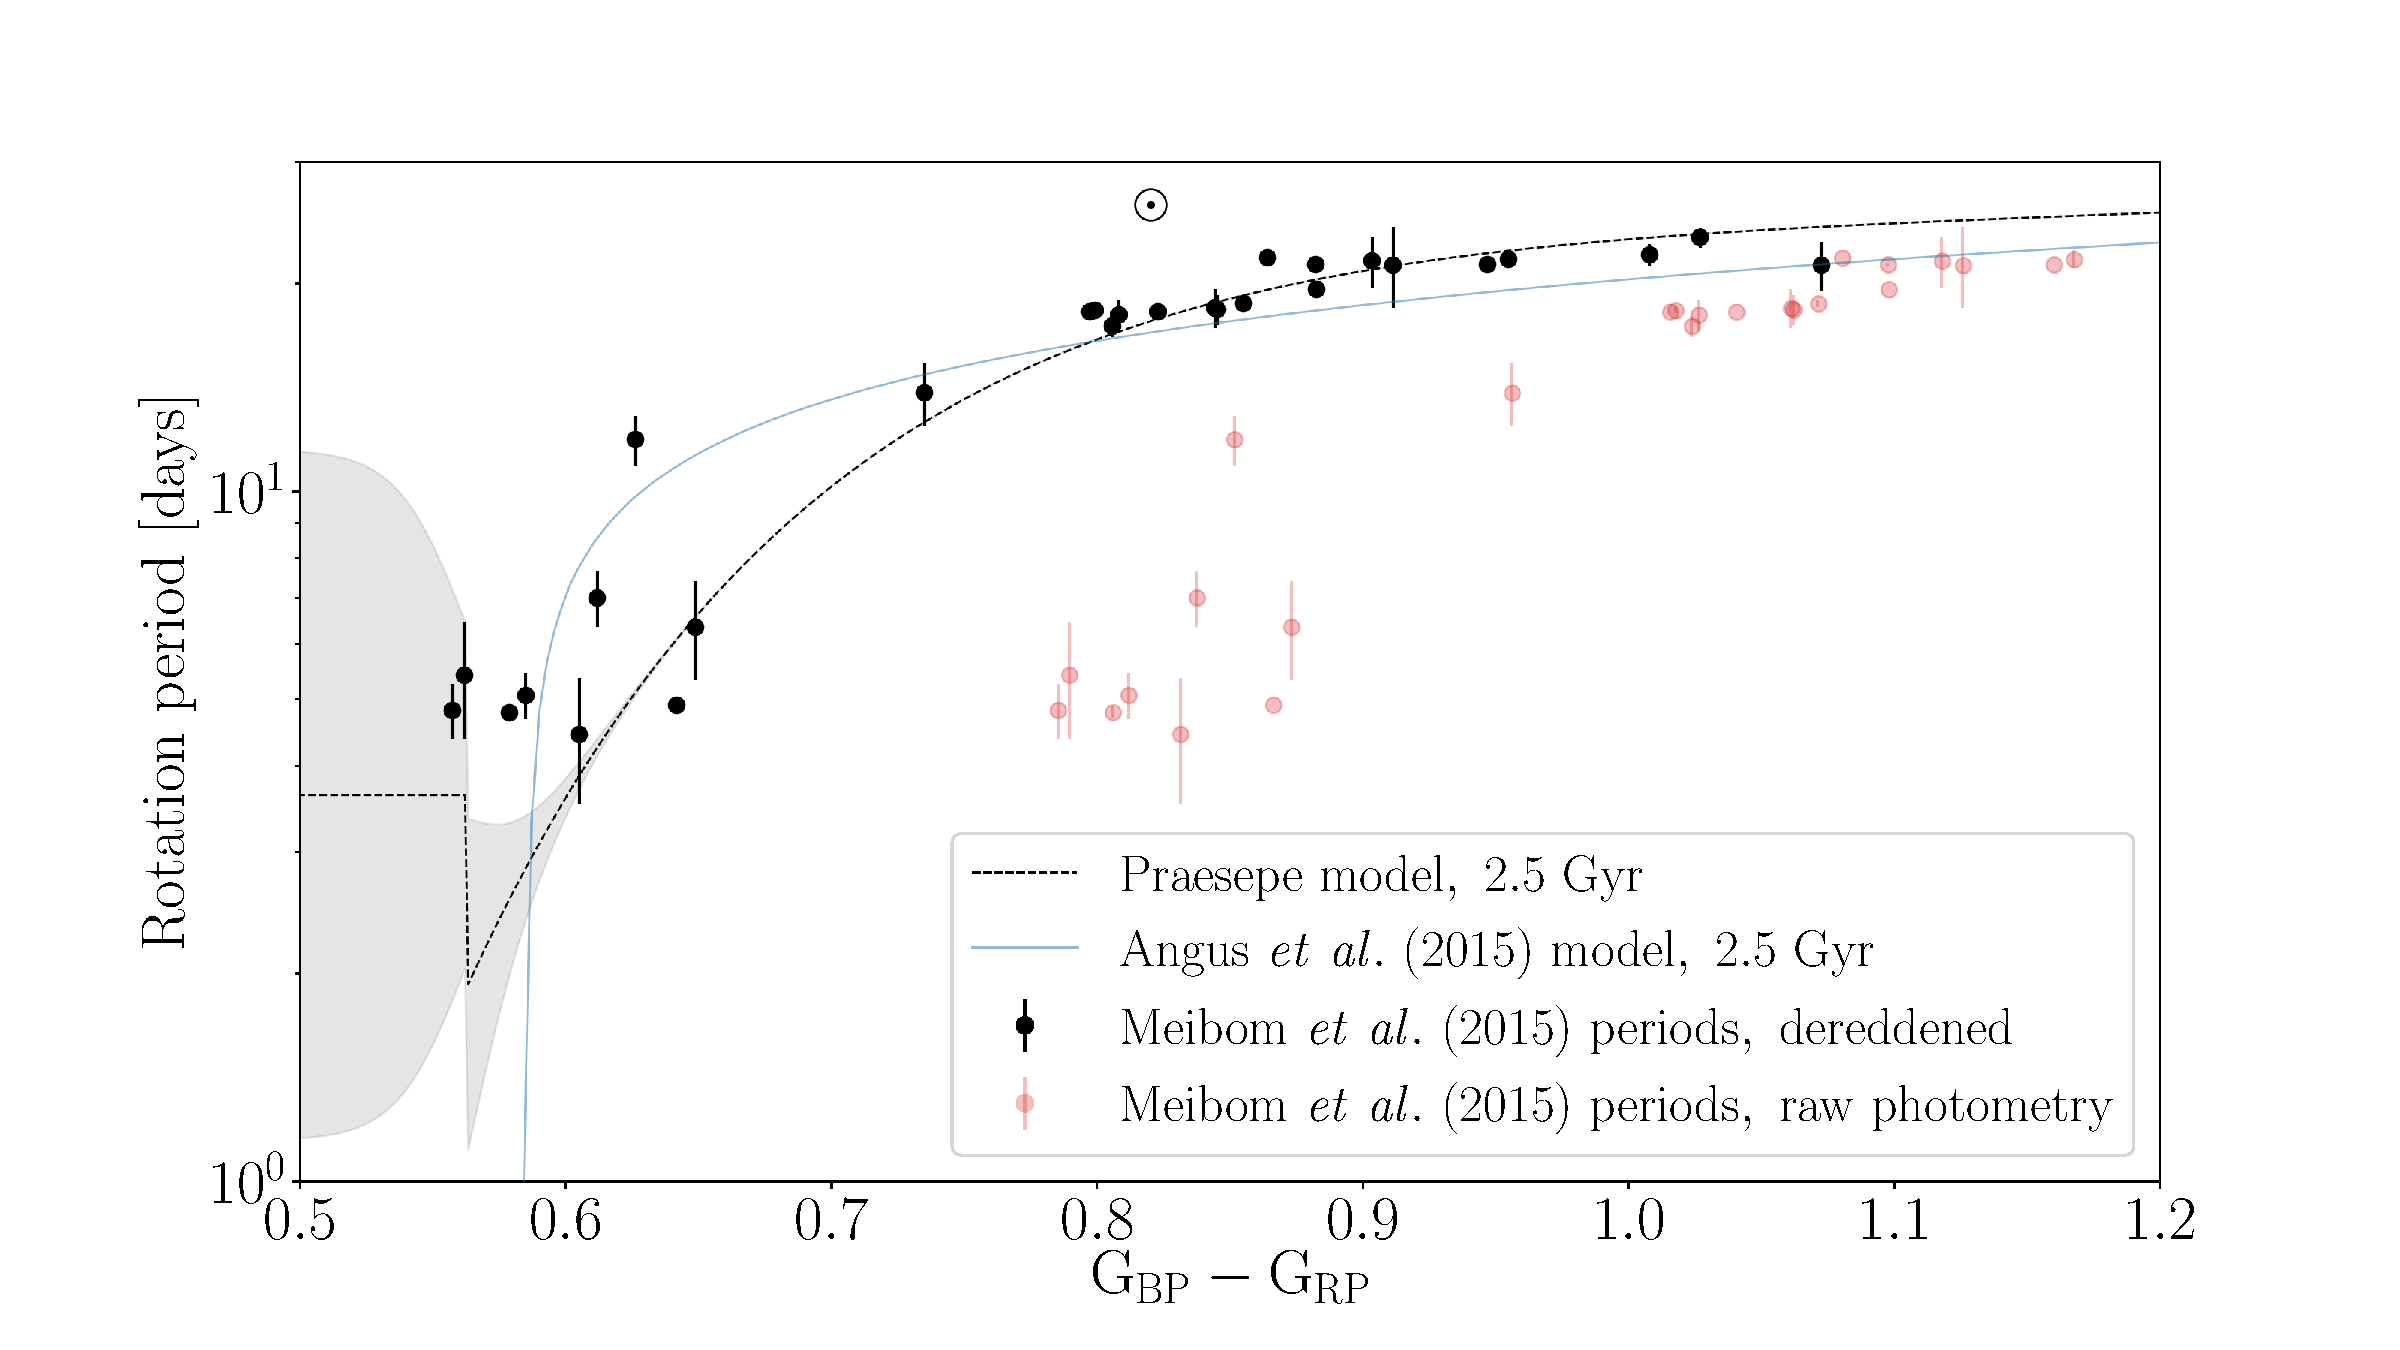
\includegraphics[width=1\textwidth]{NGC6819}
\label{fig:NGC6819}
\end{figure}

\begin{figure}
  \caption{
    The inferred ages of members of the NGC 6819 open cluster as a function of
    their \gcolor\ color.
    Black circles and red squares show the ages of stars inferred using a
    combination of isochrone fitting and gyrochronology, with a gyrochronology
    relation that was calibrated to Praesepe and the Sun.
    Black circles show ages inferred with dereddened \gaia\ $G$, $G_{BP}$ and
    $G_{RP}$ photometry and red squares show ages inferred with uncorrected,
    raw, photometry.
    Even though V-band extinction is marginalized over in the inference
    process, reddening can still bias ages.
    Blue triangles, pointing down show ages inferred using isochrone fitting
    and gyrochronology, with the \citet{angus2015} gyrochronology model.
    Orange triangles show ages inferred using isochrone fitting only.
    The ages of F stars (stars bluer than 0.7) were precisely constrained by
    isochrones and including gyrochronology makes little difference to their
    inferred ages.
    The ages of G and K dwarfs (stars redder than 0.7) were improved in both
    precision and accuracy by including gyrochronology.
    The average age of stars, inferred using the gyrochronology model
    calibrated to Praesepe and the Sun (black circles) was 2.65 $\pm$ 0.13
    which is consistent with the established cluster age.
}
  \centering
    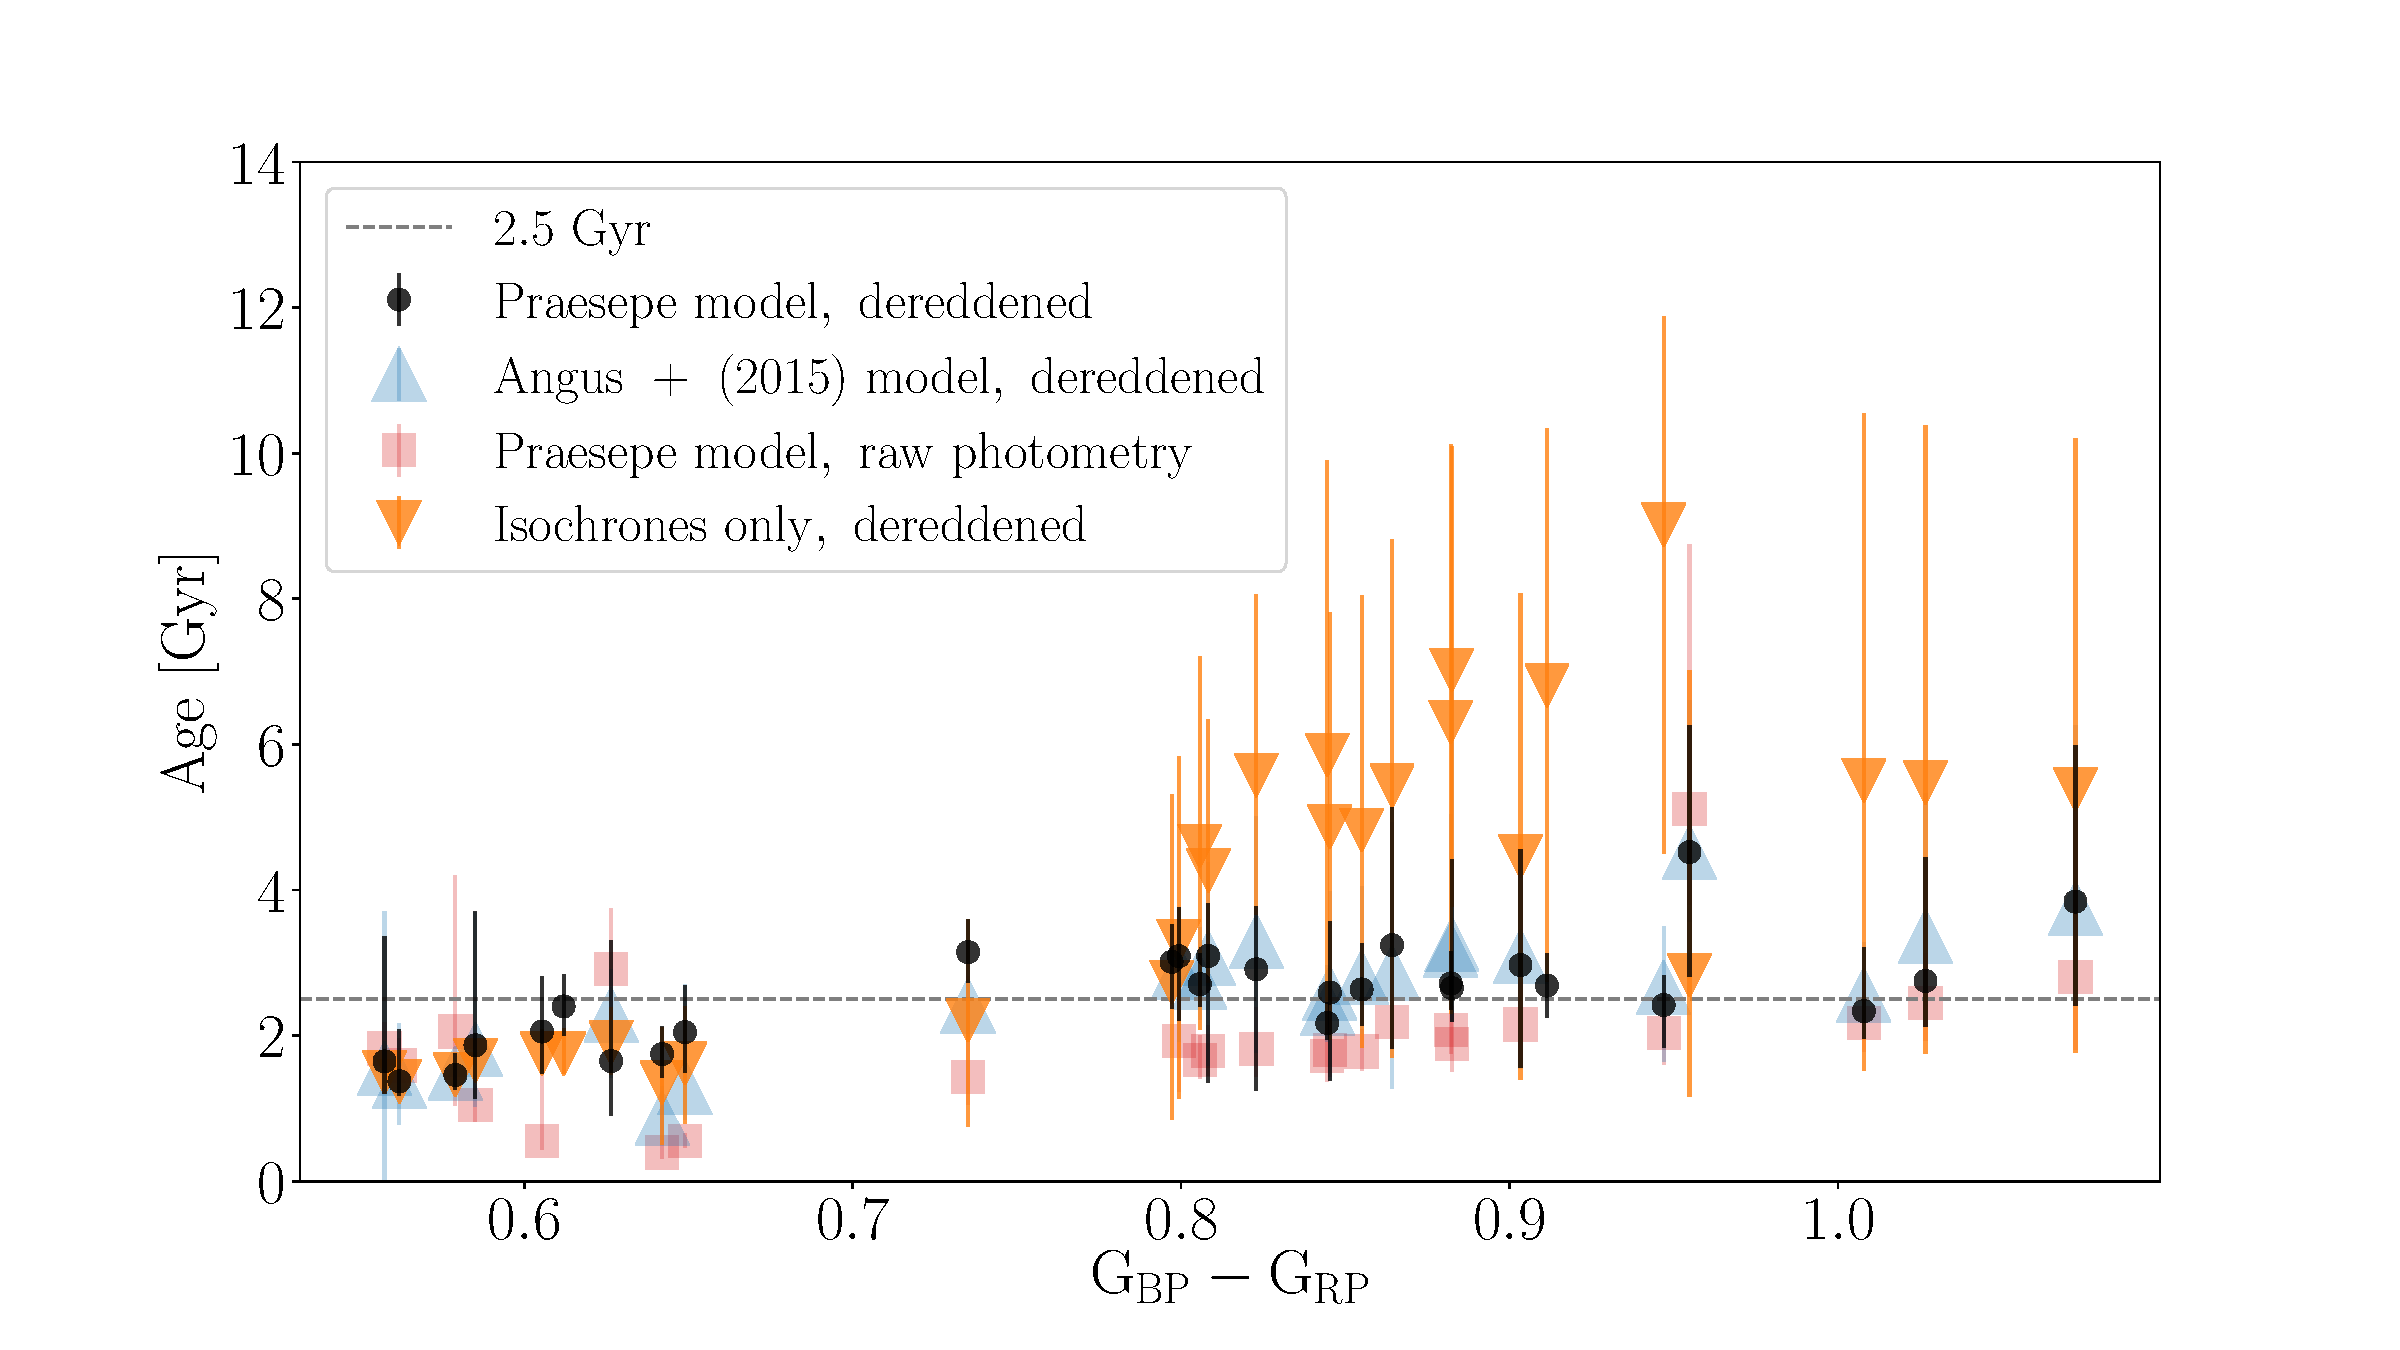
\includegraphics[width=1\textwidth]{NGC6819_results}
\label{fig:NGC6819_results}
\end{figure}

\racomment{
We found that 5\% rotation period uncertainties resulted in the most accurate
ages for NGC 6819.
The uncertainties on the measured rotation periods, provided in
\citet{meibom2015} and shown in figure \ref{fig:NGC6819}, were likely
underestimated for some stars.
Underestimated rotation period uncertainties can result in inaccurate age
estimates.
This raises the question: how should uncertainties on rotation periods be
estimated?
The likelihood is weighted by the inverse variance, so uncertainties on the
rotation period control the relative information provided by gyrochronology,
isochrones, and the prior.
If rotation period uncertainties are either too large or too small, the
resulting age estimate will be imprecise and/or inaccurate.
It is difficult to measure uncertainties on rotation periods directly:
standard techniques such as Lomb-Scargle periodograms and autocorrelation
functions do not provide them.
In general, rotation period uncertainties should probably be calculated
empirically via simulations as in the \citet{aigrain2015} study.
A thorough exploration of how rotation period uncertainties affect stellar
ages via gyrochronology is key to understanding the power of gyrochronology as
an age-dating method.
For now, we leave this exploration for a future study.
}
